\section{Organisationsplan för hela projektet}
Beställaren har beställt projektet från gruppen. Projektledaren är den medlem i gruppen som agerar mellanhand mellan projektgruppen och beställaren. Varje medlem i projektgruppen har ett ansvarsområde där han eller hon leder en arbetsgrupp bestående av delar av resten av gruppen. Det innebär att varje medlem är både arbetsledare och del i minst ett annat arbetslag. En handledare och en grupp tekniska experter finns tillgängliga om gruppen behöver hjälp att lösa något specifikt problem. Figur \ref{projektplan:organisationsplan} illustrerar strukturen.

\begin{figure}[h!]
\center
\tikzset{every picture/.style={scale=0.6}}%
% Graphic for TeX using PGF
% Title: /home/martin/TDDD77/dokumentation/projektplan/grafik/projektplan-organisationsplan.dia
% Creator: Dia v0.97.2
% CreationDate: Tue Feb 10 14:59:02 2015
% For: martin
% \usepackage{tikz}
% The following commands are not supported in PSTricks at present
% We define them conditionally, so when they are implemented,
% this pgf file will use them.
\ifx\du\undefined
  \newlength{\du}
\fi
\setlength{\du}{15\unitlength}
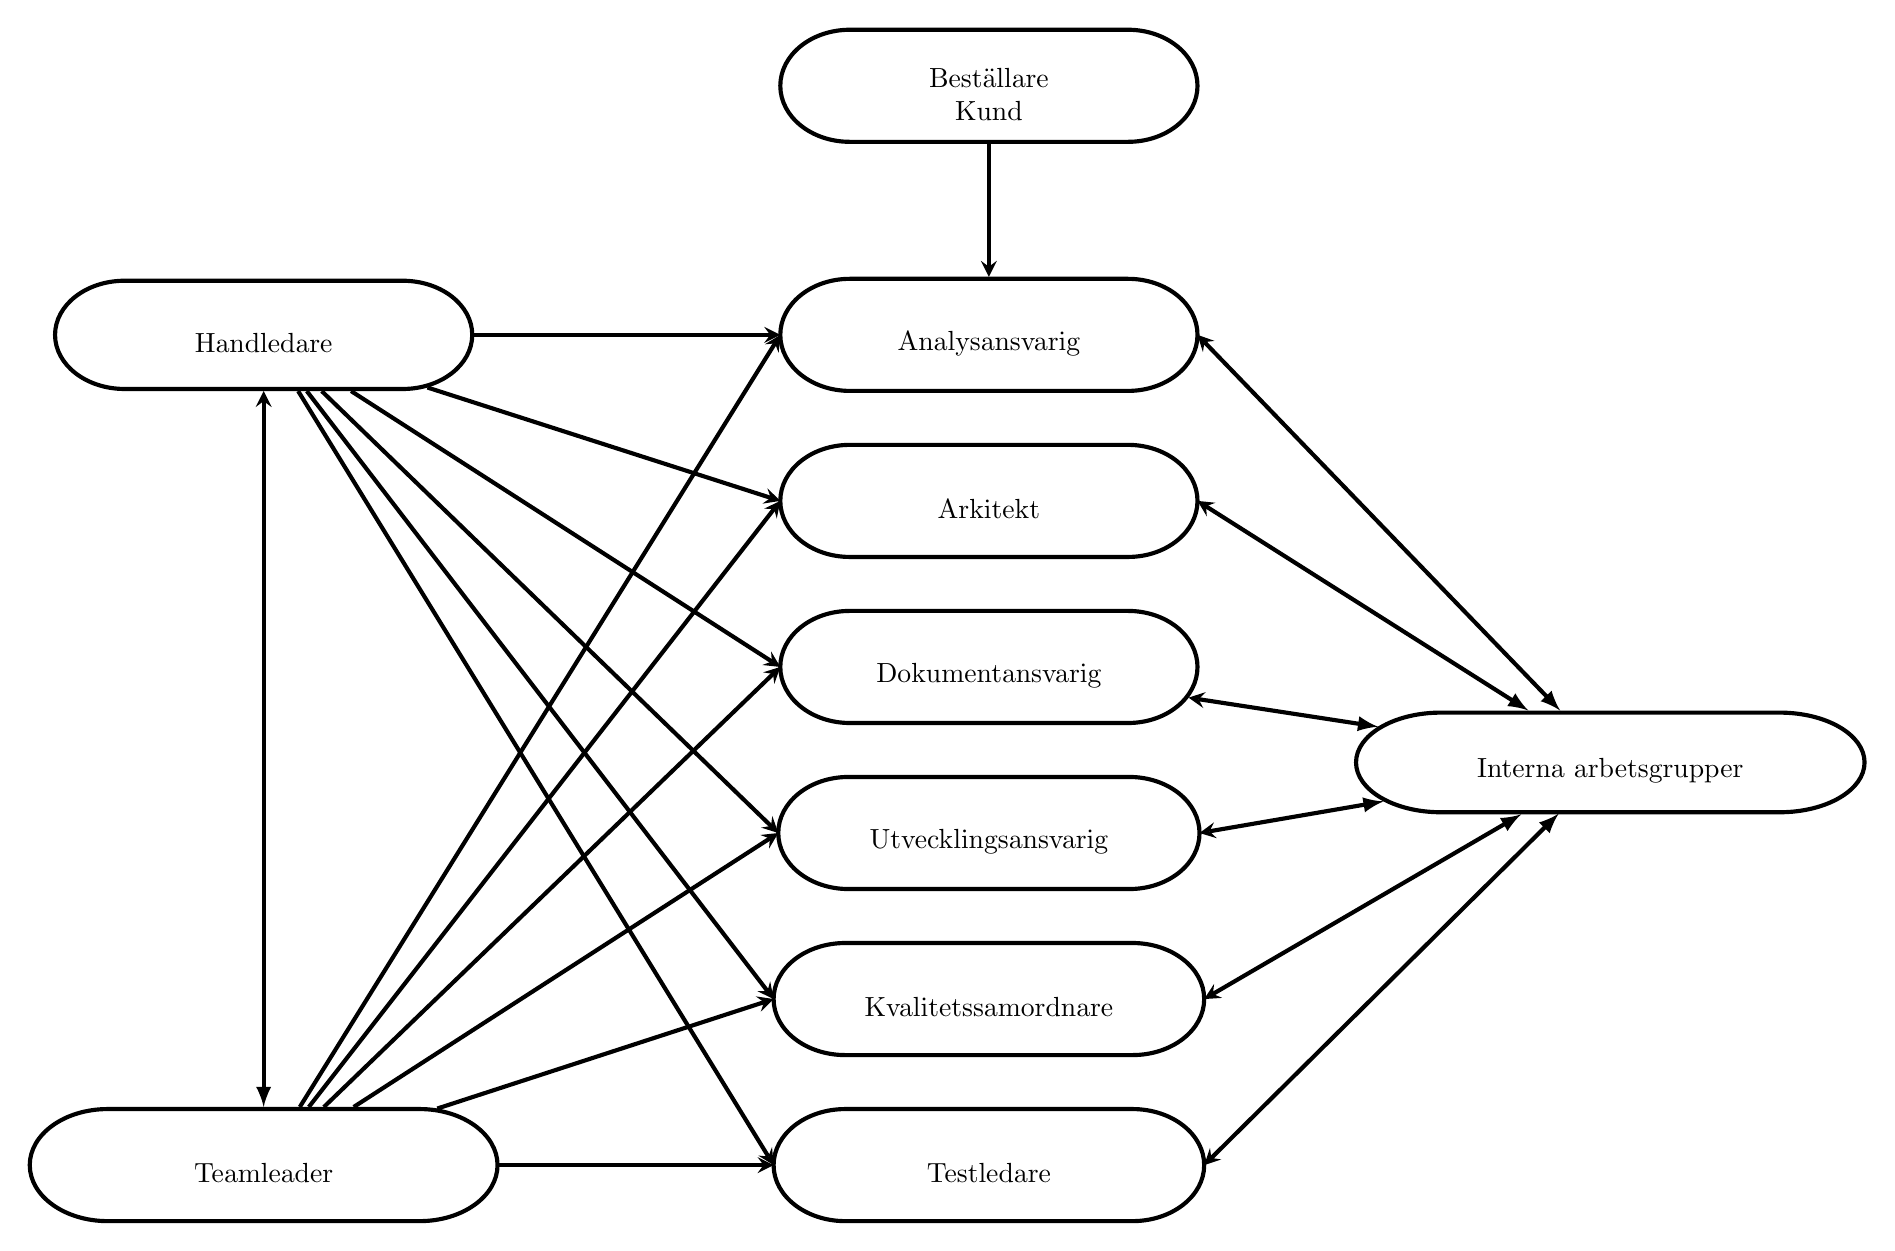
\begin{tikzpicture}
\pgftransformxscale{1.000000}
\pgftransformyscale{-1.000000}
\definecolor{dialinecolor}{rgb}{0.000000, 0.000000, 0.000000}
\pgfsetstrokecolor{dialinecolor}
\definecolor{dialinecolor}{rgb}{1.000000, 1.000000, 1.000000}
\pgfsetfillcolor{dialinecolor}
\pgfsetlinewidth{0.100000\du}
\pgfsetdash{}{0pt}
\pgfsetdash{}{0pt}
\pgfsetbuttcap
\pgfsetmiterjoin
\pgfsetlinewidth{0.100000\du}
\pgfsetbuttcap
\pgfsetmiterjoin
\pgfsetdash{}{0pt}
\definecolor{dialinecolor}{rgb}{1.000000, 1.000000, 1.000000}
\pgfsetfillcolor{dialinecolor}
\pgfpathmoveto{\pgfpoint{28.755625\du}{9.000000\du}}
\pgfpathlineto{\pgfpoint{35.455625\du}{9.000000\du}}
\pgfpathcurveto{\pgfpoint{36.380702\du}{9.000000\du}}{\pgfpoint{37.130625\du}{9.604415\du}}{\pgfpoint{37.130625\du}{10.350000\du}}
\pgfpathcurveto{\pgfpoint{37.130625\du}{11.095585\du}}{\pgfpoint{36.380702\du}{11.700000\du}}{\pgfpoint{35.455625\du}{11.700000\du}}
\pgfpathlineto{\pgfpoint{28.755625\du}{11.700000\du}}
\pgfpathcurveto{\pgfpoint{27.830548\du}{11.700000\du}}{\pgfpoint{27.080625\du}{11.095585\du}}{\pgfpoint{27.080625\du}{10.350000\du}}
\pgfpathcurveto{\pgfpoint{27.080625\du}{9.604415\du}}{\pgfpoint{27.830548\du}{9.000000\du}}{\pgfpoint{28.755625\du}{9.000000\du}}
\pgfusepath{fill}
\definecolor{dialinecolor}{rgb}{0.000000, 0.000000, 0.000000}
\pgfsetstrokecolor{dialinecolor}
\pgfpathmoveto{\pgfpoint{28.755625\du}{9.000000\du}}
\pgfpathlineto{\pgfpoint{35.455625\du}{9.000000\du}}
\pgfpathcurveto{\pgfpoint{36.380702\du}{9.000000\du}}{\pgfpoint{37.130625\du}{9.604415\du}}{\pgfpoint{37.130625\du}{10.350000\du}}
\pgfpathcurveto{\pgfpoint{37.130625\du}{11.095585\du}}{\pgfpoint{36.380702\du}{11.700000\du}}{\pgfpoint{35.455625\du}{11.700000\du}}
\pgfpathlineto{\pgfpoint{28.755625\du}{11.700000\du}}
\pgfpathcurveto{\pgfpoint{27.830548\du}{11.700000\du}}{\pgfpoint{27.080625\du}{11.095585\du}}{\pgfpoint{27.080625\du}{10.350000\du}}
\pgfpathcurveto{\pgfpoint{27.080625\du}{9.604415\du}}{\pgfpoint{27.830548\du}{9.000000\du}}{\pgfpoint{28.755625\du}{9.000000\du}}
\pgfusepath{stroke}
% setfont left to latex
\definecolor{dialinecolor}{rgb}{0.000000, 0.000000, 0.000000}
\pgfsetstrokecolor{dialinecolor}
\node at (32.105625\du,10.150000\du){Beställare};
% setfont left to latex
\definecolor{dialinecolor}{rgb}{0.000000, 0.000000, 0.000000}
\pgfsetstrokecolor{dialinecolor}
\node at (32.105625\du,10.950000\du){Kund};
\pgfsetlinewidth{0.100000\du}
\pgfsetdash{}{0pt}
\pgfsetdash{}{0pt}
\pgfsetbuttcap
\pgfsetmiterjoin
\pgfsetlinewidth{0.100000\du}
\pgfsetbuttcap
\pgfsetmiterjoin
\pgfsetdash{}{0pt}
\definecolor{dialinecolor}{rgb}{1.000000, 1.000000, 1.000000}
\pgfsetfillcolor{dialinecolor}
\pgfpathmoveto{\pgfpoint{10.878125\du}{35.000000\du}}
\pgfpathlineto{\pgfpoint{18.390625\du}{35.000000\du}}
\pgfpathcurveto{\pgfpoint{19.427885\du}{35.000000\du}}{\pgfpoint{20.268750\du}{35.604415\du}}{\pgfpoint{20.268750\du}{36.350000\du}}
\pgfpathcurveto{\pgfpoint{20.268750\du}{37.095585\du}}{\pgfpoint{19.427885\du}{37.700000\du}}{\pgfpoint{18.390625\du}{37.700000\du}}
\pgfpathlineto{\pgfpoint{10.878125\du}{37.700000\du}}
\pgfpathcurveto{\pgfpoint{9.840865\du}{37.700000\du}}{\pgfpoint{9.000000\du}{37.095585\du}}{\pgfpoint{9.000000\du}{36.350000\du}}
\pgfpathcurveto{\pgfpoint{9.000000\du}{35.604415\du}}{\pgfpoint{9.840865\du}{35.000000\du}}{\pgfpoint{10.878125\du}{35.000000\du}}
\pgfusepath{fill}
\definecolor{dialinecolor}{rgb}{0.000000, 0.000000, 0.000000}
\pgfsetstrokecolor{dialinecolor}
\pgfpathmoveto{\pgfpoint{10.878125\du}{35.000000\du}}
\pgfpathlineto{\pgfpoint{18.390625\du}{35.000000\du}}
\pgfpathcurveto{\pgfpoint{19.427885\du}{35.000000\du}}{\pgfpoint{20.268750\du}{35.604415\du}}{\pgfpoint{20.268750\du}{36.350000\du}}
\pgfpathcurveto{\pgfpoint{20.268750\du}{37.095585\du}}{\pgfpoint{19.427885\du}{37.700000\du}}{\pgfpoint{18.390625\du}{37.700000\du}}
\pgfpathlineto{\pgfpoint{10.878125\du}{37.700000\du}}
\pgfpathcurveto{\pgfpoint{9.840865\du}{37.700000\du}}{\pgfpoint{9.000000\du}{37.095585\du}}{\pgfpoint{9.000000\du}{36.350000\du}}
\pgfpathcurveto{\pgfpoint{9.000000\du}{35.604415\du}}{\pgfpoint{9.840865\du}{35.000000\du}}{\pgfpoint{10.878125\du}{35.000000\du}}
\pgfusepath{stroke}
% setfont left to latex
\definecolor{dialinecolor}{rgb}{0.000000, 0.000000, 0.000000}
\pgfsetstrokecolor{dialinecolor}
\node at (14.634375\du,36.550000\du){Teamleader};
\pgfsetlinewidth{0.100000\du}
\pgfsetdash{}{0pt}
\pgfsetdash{}{0pt}
\pgfsetbuttcap
\pgfsetmiterjoin
\pgfsetlinewidth{0.100000\du}
\pgfsetbuttcap
\pgfsetmiterjoin
\pgfsetdash{}{0pt}
\definecolor{dialinecolor}{rgb}{1.000000, 1.000000, 1.000000}
\pgfsetfillcolor{dialinecolor}
\pgfpathmoveto{\pgfpoint{11.284375\du}{15.046250\du}}
\pgfpathlineto{\pgfpoint{17.984375\du}{15.046250\du}}
\pgfpathcurveto{\pgfpoint{18.909452\du}{15.046250\du}}{\pgfpoint{19.659375\du}{15.629958\du}}{\pgfpoint{19.659375\du}{16.350000\du}}
\pgfpathcurveto{\pgfpoint{19.659375\du}{17.070042\du}}{\pgfpoint{18.909452\du}{17.653750\du}}{\pgfpoint{17.984375\du}{17.653750\du}}
\pgfpathlineto{\pgfpoint{11.284375\du}{17.653750\du}}
\pgfpathcurveto{\pgfpoint{10.359298\du}{17.653750\du}}{\pgfpoint{9.609375\du}{17.070042\du}}{\pgfpoint{9.609375\du}{16.350000\du}}
\pgfpathcurveto{\pgfpoint{9.609375\du}{15.629958\du}}{\pgfpoint{10.359298\du}{15.046250\du}}{\pgfpoint{11.284375\du}{15.046250\du}}
\pgfusepath{fill}
\definecolor{dialinecolor}{rgb}{0.000000, 0.000000, 0.000000}
\pgfsetstrokecolor{dialinecolor}
\pgfpathmoveto{\pgfpoint{11.284375\du}{15.046250\du}}
\pgfpathlineto{\pgfpoint{17.984375\du}{15.046250\du}}
\pgfpathcurveto{\pgfpoint{18.909452\du}{15.046250\du}}{\pgfpoint{19.659375\du}{15.629958\du}}{\pgfpoint{19.659375\du}{16.350000\du}}
\pgfpathcurveto{\pgfpoint{19.659375\du}{17.070042\du}}{\pgfpoint{18.909452\du}{17.653750\du}}{\pgfpoint{17.984375\du}{17.653750\du}}
\pgfpathlineto{\pgfpoint{11.284375\du}{17.653750\du}}
\pgfpathcurveto{\pgfpoint{10.359298\du}{17.653750\du}}{\pgfpoint{9.609375\du}{17.070042\du}}{\pgfpoint{9.609375\du}{16.350000\du}}
\pgfpathcurveto{\pgfpoint{9.609375\du}{15.629958\du}}{\pgfpoint{10.359298\du}{15.046250\du}}{\pgfpoint{11.284375\du}{15.046250\du}}
\pgfusepath{stroke}
% setfont left to latex
\definecolor{dialinecolor}{rgb}{0.000000, 0.000000, 0.000000}
\pgfsetstrokecolor{dialinecolor}
\node at (14.634375\du,16.550000\du){Handledare};
\pgfsetlinewidth{0.100000\du}
\pgfsetdash{}{0pt}
\pgfsetdash{}{0pt}
\pgfsetbuttcap
\pgfsetmiterjoin
\pgfsetlinewidth{0.100000\du}
\pgfsetbuttcap
\pgfsetmiterjoin
\pgfsetdash{}{0pt}
\definecolor{dialinecolor}{rgb}{1.000000, 1.000000, 1.000000}
\pgfsetfillcolor{dialinecolor}
\pgfpathmoveto{\pgfpoint{28.755625\du}{15.000000\du}}
\pgfpathlineto{\pgfpoint{35.455625\du}{15.000000\du}}
\pgfpathcurveto{\pgfpoint{36.380702\du}{15.000000\du}}{\pgfpoint{37.130625\du}{15.604415\du}}{\pgfpoint{37.130625\du}{16.350000\du}}
\pgfpathcurveto{\pgfpoint{37.130625\du}{17.095585\du}}{\pgfpoint{36.380702\du}{17.700000\du}}{\pgfpoint{35.455625\du}{17.700000\du}}
\pgfpathlineto{\pgfpoint{28.755625\du}{17.700000\du}}
\pgfpathcurveto{\pgfpoint{27.830548\du}{17.700000\du}}{\pgfpoint{27.080625\du}{17.095585\du}}{\pgfpoint{27.080625\du}{16.350000\du}}
\pgfpathcurveto{\pgfpoint{27.080625\du}{15.604415\du}}{\pgfpoint{27.830548\du}{15.000000\du}}{\pgfpoint{28.755625\du}{15.000000\du}}
\pgfusepath{fill}
\definecolor{dialinecolor}{rgb}{0.000000, 0.000000, 0.000000}
\pgfsetstrokecolor{dialinecolor}
\pgfpathmoveto{\pgfpoint{28.755625\du}{15.000000\du}}
\pgfpathlineto{\pgfpoint{35.455625\du}{15.000000\du}}
\pgfpathcurveto{\pgfpoint{36.380702\du}{15.000000\du}}{\pgfpoint{37.130625\du}{15.604415\du}}{\pgfpoint{37.130625\du}{16.350000\du}}
\pgfpathcurveto{\pgfpoint{37.130625\du}{17.095585\du}}{\pgfpoint{36.380702\du}{17.700000\du}}{\pgfpoint{35.455625\du}{17.700000\du}}
\pgfpathlineto{\pgfpoint{28.755625\du}{17.700000\du}}
\pgfpathcurveto{\pgfpoint{27.830548\du}{17.700000\du}}{\pgfpoint{27.080625\du}{17.095585\du}}{\pgfpoint{27.080625\du}{16.350000\du}}
\pgfpathcurveto{\pgfpoint{27.080625\du}{15.604415\du}}{\pgfpoint{27.830548\du}{15.000000\du}}{\pgfpoint{28.755625\du}{15.000000\du}}
\pgfusepath{stroke}
% setfont left to latex
\definecolor{dialinecolor}{rgb}{0.000000, 0.000000, 0.000000}
\pgfsetstrokecolor{dialinecolor}
\node at (32.105625\du,16.550000\du){Analysansvarig};
\pgfsetlinewidth{0.100000\du}
\pgfsetdash{}{0pt}
\pgfsetdash{}{0pt}
\pgfsetbuttcap
\pgfsetmiterjoin
\pgfsetlinewidth{0.100000\du}
\pgfsetbuttcap
\pgfsetmiterjoin
\pgfsetdash{}{0pt}
\definecolor{dialinecolor}{rgb}{1.000000, 1.000000, 1.000000}
\pgfsetfillcolor{dialinecolor}
\pgfpathmoveto{\pgfpoint{28.755625\du}{19.000000\du}}
\pgfpathlineto{\pgfpoint{35.455625\du}{19.000000\du}}
\pgfpathcurveto{\pgfpoint{36.380702\du}{19.000000\du}}{\pgfpoint{37.130625\du}{19.604415\du}}{\pgfpoint{37.130625\du}{20.350000\du}}
\pgfpathcurveto{\pgfpoint{37.130625\du}{21.095585\du}}{\pgfpoint{36.380702\du}{21.700000\du}}{\pgfpoint{35.455625\du}{21.700000\du}}
\pgfpathlineto{\pgfpoint{28.755625\du}{21.700000\du}}
\pgfpathcurveto{\pgfpoint{27.830548\du}{21.700000\du}}{\pgfpoint{27.080625\du}{21.095585\du}}{\pgfpoint{27.080625\du}{20.350000\du}}
\pgfpathcurveto{\pgfpoint{27.080625\du}{19.604415\du}}{\pgfpoint{27.830548\du}{19.000000\du}}{\pgfpoint{28.755625\du}{19.000000\du}}
\pgfusepath{fill}
\definecolor{dialinecolor}{rgb}{0.000000, 0.000000, 0.000000}
\pgfsetstrokecolor{dialinecolor}
\pgfpathmoveto{\pgfpoint{28.755625\du}{19.000000\du}}
\pgfpathlineto{\pgfpoint{35.455625\du}{19.000000\du}}
\pgfpathcurveto{\pgfpoint{36.380702\du}{19.000000\du}}{\pgfpoint{37.130625\du}{19.604415\du}}{\pgfpoint{37.130625\du}{20.350000\du}}
\pgfpathcurveto{\pgfpoint{37.130625\du}{21.095585\du}}{\pgfpoint{36.380702\du}{21.700000\du}}{\pgfpoint{35.455625\du}{21.700000\du}}
\pgfpathlineto{\pgfpoint{28.755625\du}{21.700000\du}}
\pgfpathcurveto{\pgfpoint{27.830548\du}{21.700000\du}}{\pgfpoint{27.080625\du}{21.095585\du}}{\pgfpoint{27.080625\du}{20.350000\du}}
\pgfpathcurveto{\pgfpoint{27.080625\du}{19.604415\du}}{\pgfpoint{27.830548\du}{19.000000\du}}{\pgfpoint{28.755625\du}{19.000000\du}}
\pgfusepath{stroke}
% setfont left to latex
\definecolor{dialinecolor}{rgb}{0.000000, 0.000000, 0.000000}
\pgfsetstrokecolor{dialinecolor}
\node at (32.105625\du,20.550000\du){Arkitekt};
\pgfsetlinewidth{0.100000\du}
\pgfsetdash{}{0pt}
\pgfsetdash{}{0pt}
\pgfsetbuttcap
\pgfsetmiterjoin
\pgfsetlinewidth{0.100000\du}
\pgfsetbuttcap
\pgfsetmiterjoin
\pgfsetdash{}{0pt}
\definecolor{dialinecolor}{rgb}{1.000000, 1.000000, 1.000000}
\pgfsetfillcolor{dialinecolor}
\pgfpathmoveto{\pgfpoint{28.755625\du}{23.000000\du}}
\pgfpathlineto{\pgfpoint{35.455625\du}{23.000000\du}}
\pgfpathcurveto{\pgfpoint{36.380702\du}{23.000000\du}}{\pgfpoint{37.130625\du}{23.604415\du}}{\pgfpoint{37.130625\du}{24.350000\du}}
\pgfpathcurveto{\pgfpoint{37.130625\du}{25.095585\du}}{\pgfpoint{36.380702\du}{25.700000\du}}{\pgfpoint{35.455625\du}{25.700000\du}}
\pgfpathlineto{\pgfpoint{28.755625\du}{25.700000\du}}
\pgfpathcurveto{\pgfpoint{27.830548\du}{25.700000\du}}{\pgfpoint{27.080625\du}{25.095585\du}}{\pgfpoint{27.080625\du}{24.350000\du}}
\pgfpathcurveto{\pgfpoint{27.080625\du}{23.604415\du}}{\pgfpoint{27.830548\du}{23.000000\du}}{\pgfpoint{28.755625\du}{23.000000\du}}
\pgfusepath{fill}
\definecolor{dialinecolor}{rgb}{0.000000, 0.000000, 0.000000}
\pgfsetstrokecolor{dialinecolor}
\pgfpathmoveto{\pgfpoint{28.755625\du}{23.000000\du}}
\pgfpathlineto{\pgfpoint{35.455625\du}{23.000000\du}}
\pgfpathcurveto{\pgfpoint{36.380702\du}{23.000000\du}}{\pgfpoint{37.130625\du}{23.604415\du}}{\pgfpoint{37.130625\du}{24.350000\du}}
\pgfpathcurveto{\pgfpoint{37.130625\du}{25.095585\du}}{\pgfpoint{36.380702\du}{25.700000\du}}{\pgfpoint{35.455625\du}{25.700000\du}}
\pgfpathlineto{\pgfpoint{28.755625\du}{25.700000\du}}
\pgfpathcurveto{\pgfpoint{27.830548\du}{25.700000\du}}{\pgfpoint{27.080625\du}{25.095585\du}}{\pgfpoint{27.080625\du}{24.350000\du}}
\pgfpathcurveto{\pgfpoint{27.080625\du}{23.604415\du}}{\pgfpoint{27.830548\du}{23.000000\du}}{\pgfpoint{28.755625\du}{23.000000\du}}
\pgfusepath{stroke}
% setfont left to latex
\definecolor{dialinecolor}{rgb}{0.000000, 0.000000, 0.000000}
\pgfsetstrokecolor{dialinecolor}
\node at (32.105625\du,24.550000\du){Dokumentansvarig};
\pgfsetlinewidth{0.100000\du}
\pgfsetdash{}{0pt}
\pgfsetdash{}{0pt}
\pgfsetbuttcap
\pgfsetmiterjoin
\pgfsetlinewidth{0.100000\du}
\pgfsetbuttcap
\pgfsetmiterjoin
\pgfsetdash{}{0pt}
\definecolor{dialinecolor}{rgb}{1.000000, 1.000000, 1.000000}
\pgfsetfillcolor{dialinecolor}
\pgfpathmoveto{\pgfpoint{28.723125\du}{27.000000\du}}
\pgfpathlineto{\pgfpoint{35.488125\du}{27.000000\du}}
\pgfpathcurveto{\pgfpoint{36.422177\du}{27.000000\du}}{\pgfpoint{37.179375\du}{27.604415\du}}{\pgfpoint{37.179375\du}{28.350000\du}}
\pgfpathcurveto{\pgfpoint{37.179375\du}{29.095585\du}}{\pgfpoint{36.422177\du}{29.700000\du}}{\pgfpoint{35.488125\du}{29.700000\du}}
\pgfpathlineto{\pgfpoint{28.723125\du}{29.700000\du}}
\pgfpathcurveto{\pgfpoint{27.789073\du}{29.700000\du}}{\pgfpoint{27.031875\du}{29.095585\du}}{\pgfpoint{27.031875\du}{28.350000\du}}
\pgfpathcurveto{\pgfpoint{27.031875\du}{27.604415\du}}{\pgfpoint{27.789073\du}{27.000000\du}}{\pgfpoint{28.723125\du}{27.000000\du}}
\pgfusepath{fill}
\definecolor{dialinecolor}{rgb}{0.000000, 0.000000, 0.000000}
\pgfsetstrokecolor{dialinecolor}
\pgfpathmoveto{\pgfpoint{28.723125\du}{27.000000\du}}
\pgfpathlineto{\pgfpoint{35.488125\du}{27.000000\du}}
\pgfpathcurveto{\pgfpoint{36.422177\du}{27.000000\du}}{\pgfpoint{37.179375\du}{27.604415\du}}{\pgfpoint{37.179375\du}{28.350000\du}}
\pgfpathcurveto{\pgfpoint{37.179375\du}{29.095585\du}}{\pgfpoint{36.422177\du}{29.700000\du}}{\pgfpoint{35.488125\du}{29.700000\du}}
\pgfpathlineto{\pgfpoint{28.723125\du}{29.700000\du}}
\pgfpathcurveto{\pgfpoint{27.789073\du}{29.700000\du}}{\pgfpoint{27.031875\du}{29.095585\du}}{\pgfpoint{27.031875\du}{28.350000\du}}
\pgfpathcurveto{\pgfpoint{27.031875\du}{27.604415\du}}{\pgfpoint{27.789073\du}{27.000000\du}}{\pgfpoint{28.723125\du}{27.000000\du}}
\pgfusepath{stroke}
% setfont left to latex
\definecolor{dialinecolor}{rgb}{0.000000, 0.000000, 0.000000}
\pgfsetstrokecolor{dialinecolor}
\node at (32.105625\du,28.550000\du){Utvecklingsansvarig};
\pgfsetlinewidth{0.100000\du}
\pgfsetdash{}{0pt}
\pgfsetdash{}{0pt}
\pgfsetbuttcap
\pgfsetmiterjoin
\pgfsetlinewidth{0.100000\du}
\pgfsetbuttcap
\pgfsetmiterjoin
\pgfsetdash{}{0pt}
\definecolor{dialinecolor}{rgb}{1.000000, 1.000000, 1.000000}
\pgfsetfillcolor{dialinecolor}
\pgfpathmoveto{\pgfpoint{28.648125\du}{31.000000\du}}
\pgfpathlineto{\pgfpoint{35.563125\du}{31.000000\du}}
\pgfpathcurveto{\pgfpoint{36.517888\du}{31.000000\du}}{\pgfpoint{37.291875\du}{31.604415\du}}{\pgfpoint{37.291875\du}{32.350000\du}}
\pgfpathcurveto{\pgfpoint{37.291875\du}{33.095585\du}}{\pgfpoint{36.517888\du}{33.700000\du}}{\pgfpoint{35.563125\du}{33.700000\du}}
\pgfpathlineto{\pgfpoint{28.648125\du}{33.700000\du}}
\pgfpathcurveto{\pgfpoint{27.693362\du}{33.700000\du}}{\pgfpoint{26.919375\du}{33.095585\du}}{\pgfpoint{26.919375\du}{32.350000\du}}
\pgfpathcurveto{\pgfpoint{26.919375\du}{31.604415\du}}{\pgfpoint{27.693362\du}{31.000000\du}}{\pgfpoint{28.648125\du}{31.000000\du}}
\pgfusepath{fill}
\definecolor{dialinecolor}{rgb}{0.000000, 0.000000, 0.000000}
\pgfsetstrokecolor{dialinecolor}
\pgfpathmoveto{\pgfpoint{28.648125\du}{31.000000\du}}
\pgfpathlineto{\pgfpoint{35.563125\du}{31.000000\du}}
\pgfpathcurveto{\pgfpoint{36.517888\du}{31.000000\du}}{\pgfpoint{37.291875\du}{31.604415\du}}{\pgfpoint{37.291875\du}{32.350000\du}}
\pgfpathcurveto{\pgfpoint{37.291875\du}{33.095585\du}}{\pgfpoint{36.517888\du}{33.700000\du}}{\pgfpoint{35.563125\du}{33.700000\du}}
\pgfpathlineto{\pgfpoint{28.648125\du}{33.700000\du}}
\pgfpathcurveto{\pgfpoint{27.693362\du}{33.700000\du}}{\pgfpoint{26.919375\du}{33.095585\du}}{\pgfpoint{26.919375\du}{32.350000\du}}
\pgfpathcurveto{\pgfpoint{26.919375\du}{31.604415\du}}{\pgfpoint{27.693362\du}{31.000000\du}}{\pgfpoint{28.648125\du}{31.000000\du}}
\pgfusepath{stroke}
% setfont left to latex
\definecolor{dialinecolor}{rgb}{0.000000, 0.000000, 0.000000}
\pgfsetstrokecolor{dialinecolor}
\node at (32.105625\du,32.550000\du){Kvalitetssamordnare};
\pgfsetlinewidth{0.100000\du}
\pgfsetdash{}{0pt}
\pgfsetdash{}{0pt}
\pgfsetbuttcap
{
\definecolor{dialinecolor}{rgb}{0.000000, 0.000000, 0.000000}
\pgfsetfillcolor{dialinecolor}
% was here!!!
\pgfsetarrowsstart{stealth}
\definecolor{dialinecolor}{rgb}{0.000000, 0.000000, 0.000000}
\pgfsetstrokecolor{dialinecolor}
\draw (27.080625\du,16.350000\du)--(15.505324\du,34.950464\du);
}
\pgfsetlinewidth{0.100000\du}
\pgfsetdash{}{0pt}
\pgfsetdash{}{0pt}
\pgfsetbuttcap
{
\definecolor{dialinecolor}{rgb}{0.000000, 0.000000, 0.000000}
\pgfsetfillcolor{dialinecolor}
% was here!!!
\pgfsetarrowsstart{stealth}
\definecolor{dialinecolor}{rgb}{0.000000, 0.000000, 0.000000}
\pgfsetstrokecolor{dialinecolor}
\draw (27.080625\du,20.350000\du)--(15.722966\du,34.950586\du);
}
\pgfsetlinewidth{0.100000\du}
\pgfsetdash{}{0pt}
\pgfsetdash{}{0pt}
\pgfsetbuttcap
{
\definecolor{dialinecolor}{rgb}{0.000000, 0.000000, 0.000000}
\pgfsetfillcolor{dialinecolor}
% was here!!!
\pgfsetarrowsstart{stealth}
\definecolor{dialinecolor}{rgb}{0.000000, 0.000000, 0.000000}
\pgfsetstrokecolor{dialinecolor}
\draw (27.080625\du,24.350000\du)--(16.083804\du,34.952539\du);
}
\pgfsetlinewidth{0.100000\du}
\pgfsetdash{}{0pt}
\pgfsetdash{}{0pt}
\pgfsetbuttcap
{
\definecolor{dialinecolor}{rgb}{0.000000, 0.000000, 0.000000}
\pgfsetfillcolor{dialinecolor}
% was here!!!
\pgfsetarrowsstart{stealth}
\definecolor{dialinecolor}{rgb}{0.000000, 0.000000, 0.000000}
\pgfsetstrokecolor{dialinecolor}
\draw (27.031875\du,28.350000\du)--(16.803029\du,34.950586\du);
}
\pgfsetlinewidth{0.100000\du}
\pgfsetdash{}{0pt}
\pgfsetdash{}{0pt}
\pgfsetbuttcap
{
\definecolor{dialinecolor}{rgb}{0.000000, 0.000000, 0.000000}
\pgfsetfillcolor{dialinecolor}
% was here!!!
\pgfsetarrowsstart{stealth}
\definecolor{dialinecolor}{rgb}{0.000000, 0.000000, 0.000000}
\pgfsetstrokecolor{dialinecolor}
\draw (26.919375\du,32.350000\du)--(18.816854\du,34.988184\du);
}
\pgfsetlinewidth{0.100000\du}
\pgfsetdash{}{0pt}
\pgfsetdash{}{0pt}
\pgfsetbuttcap
\pgfsetmiterjoin
\pgfsetlinewidth{0.100000\du}
\pgfsetbuttcap
\pgfsetmiterjoin
\pgfsetdash{}{0pt}
\definecolor{dialinecolor}{rgb}{1.000000, 1.000000, 1.000000}
\pgfsetfillcolor{dialinecolor}
\pgfpathmoveto{\pgfpoint{42.991667\du}{25.449997\du}}
\pgfpathlineto{\pgfpoint{51.158334\du}{25.449997\du}}
\pgfpathcurveto{\pgfpoint{52.285916\du}{25.449997\du}}{\pgfpoint{53.200000\du}{25.987255\du}}{\pgfpoint{53.200000\du}{26.649997\du}}
\pgfpathcurveto{\pgfpoint{53.200000\du}{27.312739\du}}{\pgfpoint{52.285916\du}{27.849997\du}}{\pgfpoint{51.158334\du}{27.849997\du}}
\pgfpathlineto{\pgfpoint{42.991667\du}{27.849997\du}}
\pgfpathcurveto{\pgfpoint{41.864085\du}{27.849997\du}}{\pgfpoint{40.950000\du}{27.312739\du}}{\pgfpoint{40.950000\du}{26.649997\du}}
\pgfpathcurveto{\pgfpoint{40.950000\du}{25.987255\du}}{\pgfpoint{41.864085\du}{25.449997\du}}{\pgfpoint{42.991667\du}{25.449997\du}}
\pgfusepath{fill}
\definecolor{dialinecolor}{rgb}{0.000000, 0.000000, 0.000000}
\pgfsetstrokecolor{dialinecolor}
\pgfpathmoveto{\pgfpoint{42.991667\du}{25.449997\du}}
\pgfpathlineto{\pgfpoint{51.158334\du}{25.449997\du}}
\pgfpathcurveto{\pgfpoint{52.285916\du}{25.449997\du}}{\pgfpoint{53.200000\du}{25.987255\du}}{\pgfpoint{53.200000\du}{26.649997\du}}
\pgfpathcurveto{\pgfpoint{53.200000\du}{27.312739\du}}{\pgfpoint{52.285916\du}{27.849997\du}}{\pgfpoint{51.158334\du}{27.849997\du}}
\pgfpathlineto{\pgfpoint{42.991667\du}{27.849997\du}}
\pgfpathcurveto{\pgfpoint{41.864085\du}{27.849997\du}}{\pgfpoint{40.950000\du}{27.312739\du}}{\pgfpoint{40.950000\du}{26.649997\du}}
\pgfpathcurveto{\pgfpoint{40.950000\du}{25.987255\du}}{\pgfpoint{41.864085\du}{25.449997\du}}{\pgfpoint{42.991667\du}{25.449997\du}}
\pgfusepath{stroke}
% setfont left to latex
\definecolor{dialinecolor}{rgb}{0.000000, 0.000000, 0.000000}
\pgfsetstrokecolor{dialinecolor}
\node at (47.075000\du,26.849997\du){Interna arbetsgrupper};
% setfont left to latex
\definecolor{dialinecolor}{rgb}{0.000000, 0.000000, 0.000000}
\pgfsetstrokecolor{dialinecolor}
\node[anchor=west] at (14.634375\du,36.350000\du){};
\pgfsetlinewidth{0.100000\du}
\pgfsetdash{}{0pt}
\pgfsetdash{}{0pt}
\pgfsetbuttcap
{
\definecolor{dialinecolor}{rgb}{0.000000, 0.000000, 0.000000}
\pgfsetfillcolor{dialinecolor}
% was here!!!
\pgfsetarrowsstart{stealth}
\definecolor{dialinecolor}{rgb}{0.000000, 0.000000, 0.000000}
\pgfsetstrokecolor{dialinecolor}
\draw (32.105625\du,14.952539\du)--(32.105625\du,11.747461\du);
}
\pgfsetlinewidth{0.100000\du}
\pgfsetdash{}{0pt}
\pgfsetdash{}{0pt}
\pgfsetbuttcap
{
\definecolor{dialinecolor}{rgb}{0.000000, 0.000000, 0.000000}
\pgfsetfillcolor{dialinecolor}
% was here!!!
\pgfsetarrowsstart{stealth}
\definecolor{dialinecolor}{rgb}{0.000000, 0.000000, 0.000000}
\pgfsetstrokecolor{dialinecolor}
\draw (27.080401\du,16.350000\du)--(19.659599\du,16.350000\du);
}
\pgfsetlinewidth{0.100000\du}
\pgfsetdash{}{0pt}
\pgfsetdash{}{0pt}
\pgfsetbuttcap
{
\definecolor{dialinecolor}{rgb}{0.000000, 0.000000, 0.000000}
\pgfsetfillcolor{dialinecolor}
% was here!!!
\pgfsetarrowsstart{stealth}
\definecolor{dialinecolor}{rgb}{0.000000, 0.000000, 0.000000}
\pgfsetstrokecolor{dialinecolor}
\draw (27.080625\du,20.350000\du)--(18.580043\du,17.618066\du);
}
\pgfsetlinewidth{0.100000\du}
\pgfsetdash{}{0pt}
\pgfsetdash{}{0pt}
\pgfsetbuttcap
{
\definecolor{dialinecolor}{rgb}{0.000000, 0.000000, 0.000000}
\pgfsetfillcolor{dialinecolor}
% was here!!!
\pgfsetarrowsstart{stealth}
\definecolor{dialinecolor}{rgb}{0.000000, 0.000000, 0.000000}
\pgfsetstrokecolor{dialinecolor}
\draw (27.080625\du,24.350000\du)--(16.740909\du,17.704004\du);
}
\pgfsetlinewidth{0.100000\du}
\pgfsetdash{}{0pt}
\pgfsetdash{}{0pt}
\pgfsetbuttcap
{
\definecolor{dialinecolor}{rgb}{0.000000, 0.000000, 0.000000}
\pgfsetfillcolor{dialinecolor}
% was here!!!
\pgfsetarrowsstart{stealth}
\definecolor{dialinecolor}{rgb}{0.000000, 0.000000, 0.000000}
\pgfsetstrokecolor{dialinecolor}
\draw (27.031875\du,28.350000\du)--(16.033104\du,17.703882\du);
}
\pgfsetlinewidth{0.100000\du}
\pgfsetdash{}{0pt}
\pgfsetdash{}{0pt}
\pgfsetbuttcap
{
\definecolor{dialinecolor}{rgb}{0.000000, 0.000000, 0.000000}
\pgfsetfillcolor{dialinecolor}
% was here!!!
\pgfsetarrowsstart{stealth}
\definecolor{dialinecolor}{rgb}{0.000000, 0.000000, 0.000000}
\pgfsetstrokecolor{dialinecolor}
\draw (26.919375\du,32.350000\du)--(15.673996\du,17.704004\du);
}
\pgfsetlinewidth{0.100000\du}
\pgfsetdash{}{0pt}
\pgfsetdash{}{0pt}
\pgfsetbuttcap
\pgfsetmiterjoin
\pgfsetlinewidth{0.100000\du}
\pgfsetbuttcap
\pgfsetmiterjoin
\pgfsetdash{}{0pt}
\definecolor{dialinecolor}{rgb}{1.000000, 1.000000, 1.000000}
\pgfsetfillcolor{dialinecolor}
\pgfpathmoveto{\pgfpoint{28.648125\du}{35.000000\du}}
\pgfpathlineto{\pgfpoint{35.563125\du}{35.000000\du}}
\pgfpathcurveto{\pgfpoint{36.517888\du}{35.000000\du}}{\pgfpoint{37.291875\du}{35.604415\du}}{\pgfpoint{37.291875\du}{36.350000\du}}
\pgfpathcurveto{\pgfpoint{37.291875\du}{37.095585\du}}{\pgfpoint{36.517888\du}{37.700000\du}}{\pgfpoint{35.563125\du}{37.700000\du}}
\pgfpathlineto{\pgfpoint{28.648125\du}{37.700000\du}}
\pgfpathcurveto{\pgfpoint{27.693362\du}{37.700000\du}}{\pgfpoint{26.919375\du}{37.095585\du}}{\pgfpoint{26.919375\du}{36.350000\du}}
\pgfpathcurveto{\pgfpoint{26.919375\du}{35.604415\du}}{\pgfpoint{27.693362\du}{35.000000\du}}{\pgfpoint{28.648125\du}{35.000000\du}}
\pgfusepath{fill}
\definecolor{dialinecolor}{rgb}{0.000000, 0.000000, 0.000000}
\pgfsetstrokecolor{dialinecolor}
\pgfpathmoveto{\pgfpoint{28.648125\du}{35.000000\du}}
\pgfpathlineto{\pgfpoint{35.563125\du}{35.000000\du}}
\pgfpathcurveto{\pgfpoint{36.517888\du}{35.000000\du}}{\pgfpoint{37.291875\du}{35.604415\du}}{\pgfpoint{37.291875\du}{36.350000\du}}
\pgfpathcurveto{\pgfpoint{37.291875\du}{37.095585\du}}{\pgfpoint{36.517888\du}{37.700000\du}}{\pgfpoint{35.563125\du}{37.700000\du}}
\pgfpathlineto{\pgfpoint{28.648125\du}{37.700000\du}}
\pgfpathcurveto{\pgfpoint{27.693362\du}{37.700000\du}}{\pgfpoint{26.919375\du}{37.095585\du}}{\pgfpoint{26.919375\du}{36.350000\du}}
\pgfpathcurveto{\pgfpoint{26.919375\du}{35.604415\du}}{\pgfpoint{27.693362\du}{35.000000\du}}{\pgfpoint{28.648125\du}{35.000000\du}}
\pgfusepath{stroke}
% setfont left to latex
\definecolor{dialinecolor}{rgb}{0.000000, 0.000000, 0.000000}
\pgfsetstrokecolor{dialinecolor}
\node at (32.105625\du,36.550000\du){Testledare};
\pgfsetlinewidth{0.100000\du}
\pgfsetdash{}{0pt}
\pgfsetdash{}{0pt}
\pgfsetbuttcap
{
\definecolor{dialinecolor}{rgb}{0.000000, 0.000000, 0.000000}
\pgfsetfillcolor{dialinecolor}
% was here!!!
\pgfsetarrowsstart{stealth}
\definecolor{dialinecolor}{rgb}{0.000000, 0.000000, 0.000000}
\pgfsetstrokecolor{dialinecolor}
\draw (26.919375\du,36.350000\du)--(20.268874\du,36.350000\du);
}
\pgfsetlinewidth{0.100000\du}
\pgfsetdash{}{0pt}
\pgfsetdash{}{0pt}
\pgfsetbuttcap
{
\definecolor{dialinecolor}{rgb}{0.000000, 0.000000, 0.000000}
\pgfsetfillcolor{dialinecolor}
% was here!!!
\pgfsetarrowsstart{stealth}
\definecolor{dialinecolor}{rgb}{0.000000, 0.000000, 0.000000}
\pgfsetstrokecolor{dialinecolor}
\draw (26.919375\du,36.350000\du)--(15.465547\du,17.703149\du);
}
\pgfsetlinewidth{0.100000\du}
\pgfsetdash{}{0pt}
\pgfsetdash{}{0pt}
\pgfsetbuttcap
{
\definecolor{dialinecolor}{rgb}{0.000000, 0.000000, 0.000000}
\pgfsetfillcolor{dialinecolor}
% was here!!!
\pgfsetarrowsstart{stealth}
\pgfsetarrowsend{latex}
\definecolor{dialinecolor}{rgb}{0.000000, 0.000000, 0.000000}
\pgfsetstrokecolor{dialinecolor}
\draw (37.130625\du,16.350000\du)--(45.868067\du,25.399902\du);
}
\pgfsetlinewidth{0.100000\du}
\pgfsetdash{}{0pt}
\pgfsetdash{}{0pt}
\pgfsetbuttcap
{
\definecolor{dialinecolor}{rgb}{0.000000, 0.000000, 0.000000}
\pgfsetfillcolor{dialinecolor}
% was here!!!
\pgfsetarrowsstart{stealth}
\pgfsetarrowsend{latex}
\definecolor{dialinecolor}{rgb}{0.000000, 0.000000, 0.000000}
\pgfsetstrokecolor{dialinecolor}
\draw (37.130625\du,20.350000\du)--(45.102392\du,25.400303\du);
}
\pgfsetlinewidth{0.100000\du}
\pgfsetdash{}{0pt}
\pgfsetdash{}{0pt}
\pgfsetbuttcap
{
\definecolor{dialinecolor}{rgb}{0.000000, 0.000000, 0.000000}
\pgfsetfillcolor{dialinecolor}
% was here!!!
\pgfsetarrowsstart{stealth}
\pgfsetarrowsend{latex}
\definecolor{dialinecolor}{rgb}{0.000000, 0.000000, 0.000000}
\pgfsetstrokecolor{dialinecolor}
\draw (36.915578\du,25.089034\du)--(41.483412\du,25.790867\du);
}
\pgfsetlinewidth{0.100000\du}
\pgfsetdash{}{0pt}
\pgfsetdash{}{0pt}
\pgfsetbuttcap
{
\definecolor{dialinecolor}{rgb}{0.000000, 0.000000, 0.000000}
\pgfsetfillcolor{dialinecolor}
% was here!!!
\pgfsetarrowsstart{stealth}
\pgfsetarrowsend{latex}
\definecolor{dialinecolor}{rgb}{0.000000, 0.000000, 0.000000}
\pgfsetstrokecolor{dialinecolor}
\draw (37.179375\du,28.350000\du)--(41.614408\du,27.588091\du);
}
\pgfsetlinewidth{0.100000\du}
\pgfsetdash{}{0pt}
\pgfsetdash{}{0pt}
\pgfsetbuttcap
{
\definecolor{dialinecolor}{rgb}{0.000000, 0.000000, 0.000000}
\pgfsetfillcolor{dialinecolor}
% was here!!!
\pgfsetarrowsstart{stealth}
\pgfsetarrowsend{latex}
\definecolor{dialinecolor}{rgb}{0.000000, 0.000000, 0.000000}
\pgfsetstrokecolor{dialinecolor}
\draw (37.291875\du,32.350000\du)--(44.929568\du,27.900004\du);
}
\pgfsetlinewidth{0.100000\du}
\pgfsetdash{}{0pt}
\pgfsetdash{}{0pt}
\pgfsetbuttcap
{
\definecolor{dialinecolor}{rgb}{0.000000, 0.000000, 0.000000}
\pgfsetfillcolor{dialinecolor}
% was here!!!
\pgfsetarrowsstart{stealth}
\pgfsetarrowsend{latex}
\definecolor{dialinecolor}{rgb}{0.000000, 0.000000, 0.000000}
\pgfsetstrokecolor{dialinecolor}
\draw (37.291875\du,36.350000\du)--(45.833002\du,27.881442\du);
}
\pgfsetlinewidth{0.100000\du}
\pgfsetdash{}{0pt}
\pgfsetdash{}{0pt}
\pgfsetbuttcap
{
\definecolor{dialinecolor}{rgb}{0.000000, 0.000000, 0.000000}
\pgfsetfillcolor{dialinecolor}
% was here!!!
\pgfsetarrowsstart{stealth}
\pgfsetarrowsend{latex}
\definecolor{dialinecolor}{rgb}{0.000000, 0.000000, 0.000000}
\pgfsetstrokecolor{dialinecolor}
\draw (14.634375\du,17.703149\du)--(14.634375\du,34.950464\du);
}
\end{tikzpicture}

\tikzset{every picture/.style={scale=1}}%
\caption{Schema över organisationen.} \label{projektplan:organisationsplan}
\endcenter
\end{figure}

\subsection{Villkor för samarbete inom projektgruppen}
Inom gruppen har vi kommit överens om att följande gäller:
\begin{itemize}
\item{Alla skall komma väl förberedda till möten.}
\item{Meddela i tid om man inte kan närvara vid ett möte. Vid sjukdom skall detta meddelas snarast.}
\item{Man skall delta vid möten som gruppen kommit överens om.}
\item{Om man är osäker på något skall resten av gruppen alternativt experter tillfrågas om råd.}
\item{Om någon inte bidrar tillräckligt till projektet så har resterande gruppmedlemmar rätt att diskutera detta med beställaren.}
\item{Innan expert bokas skall gruppen tillfrågas i händelse att någon annan har frågor till samma expert.}
\end{itemize}

\newpage
\subsection{Ansvarsområden}
Varje gruppmedlem är huvudansvarig för olika delar av arbetet enligt tabell \ref{projektplan:ansvarsomraden}.

\begin{table}[h]
  \centering
    \begin{tabularx}{\textwidth}{| l | X | l |}
      \hline
      \textbf{Titel} & \textbf{Ansvarsområde} & \textbf{Vem} \\
      \hline
      {Projektledare} & {Ansvarig för att arbetet fortskrider enligt tidsplanen. Huvudsaklig kontaktperson för gruppen. Sköter kontakt med beställare och handledare, sammankallar möten, ordförande i gruppmöten, ansvarig för att tids- och statusrapporter skrivs och lämnas i tid.} & {PK} \\\hline
      {Dokumentansvarig} & {Ansvarig för att all dokumentation skrivs och är välformaterad.} & {HS} \\\hline
      {Mjukvaruansvarig} & {Huvudsakligen ansvarig för mjukvara på Beagleboard och PC.} & {MS} \\\hline
      {Hårdvaruansvarig} & {Ansvarig för att all hårdvara är rätt, bra virad och fungerar korrekt.} & {AY} \\\hline
      {Testansvarig} & {Ansvarig för att alla delsystem testas ingående och fungerar korrekt. Ansvarig för att systemet som helhet testas ingående.} & {DL} \\\hline
      {Leveransansvarig} & {Ansvarig för att alla leveranser sker i tid.} & {DW} \\\hline
    \end{tabularx}
  \caption{Ansvarsområden} \label{projektplan:ansvarsomraden}
\end{table}
